\documentclass[aspectratio=169, table]{beamer}

\usepackage{listings}

\lstdefinestyle{RustStyle}{
	language=Java,
	morekeywords={println, Ok, async, fn, main, use, let, mut},
	basicstyle=\ttfamily\scriptsize,
	keywordstyle=\color{blue},
	commentstyle=\color{gray},
	stringstyle=\color{red},
	breaklines=true,
	showstringspaces=false,
	tabsize=2,
	captionpos=b,
	numbers=left,
	numberstyle=\tiny\color{gray},
	frame=lines,
	backgroundcolor=\color{lightgray!10},
	comment=[l]{//},
	morecomment=[s]{/*}{*/},
	commentstyle=\color{gray}\ttfamily,
	string=[s]{'}{'},
	morestring=[s]{"}{"},
	stringstyle=\color{teal}\ttfamily,
	%	showstringspaces=false
	literate=
	{\{}{{\textcolor{red}{\{}}}1
	{\}}{{\textcolor{red}{\}}}}1
	{:}{{\textcolor{red}{:}}}1
	{=}{{\textcolor{red}{=}}}1
	{.}{{\textcolor{red}{.}}}1
	{]}{{\textcolor{red}{]}}}1
	{[}{{\textcolor{red}{[}}}1
	{\#}{{\textcolor{red}{\#}}}1
	{;}{{\textcolor{red}{;}}}1
	{?}{{\textcolor{red}{?}}}1
	{!}{{\textcolor{red}{!}}}1
}

%\usepackage[beamertheme=./praditatheme]{Pradita}

\usetheme{Pradita}

\lstdefinelanguage{bash} {
	keywords={},
	basicstyle=\ttfamily\small,
	keywordstyle=\color{blue}\bfseries,
	ndkeywords={iex},
	ndkeywordstyle=\color{purple}\bfseries,
	sensitive=true,
	commentstyle=\color{gray},
	stringstyle=\color{red},
	numbers=left,
	numberstyle=\tiny\color{gray},
	breaklines=true,
	frame=lines,
	backgroundcolor=\color{lightgray!10},
	tabsize=2,
	comment=[l]{\#},
	morecomment=[s]{/*}{*/},
	commentstyle=\color{gray}\ttfamily,
	stringstyle=\color{purple}\ttfamily,
	showstringspaces=false
}

\lstdefinestyle{JavaStyle}{
	language=Java,
	basicstyle=\ttfamily\footnotesize,
	morekeywords={String, int},
	keywordstyle=\color{blue},
	commentstyle=\color{gray},
	stringstyle=\color{red},
	breaklines=true,
	showstringspaces=false,
	tabsize=2,
	captionpos=b,
	numbers=left,
	numberstyle=\tiny\color{gray},
	frame=lines,
	backgroundcolor=\color{lightgray!10},
	comment=[l]{//},
	morecomment=[s]{/*}{*/},
	commentstyle=\color{gray}\ttfamily,
	string=[s]{'}{'},
	morestring=[s]{"}{"},
	%	stringstyle=\color{teal}\ttfamily,
	%	showstringspaces=false
}

\title{\Huge Space-based\\Architecture\\\vspace{10pt}}
\subtitle{IF231303-Software Architecture}
\author{\textbf{Alfa Yohannis}}
\begin{document}
	
	\frame{\titlepage}
	
	\begin{frame}[fragile]
		\frametitle{Contents}
		\vspace{20pt}
		\begin{columns}[t]
			\column{0.5\textwidth}
			\tableofcontents[sections={1-4}]
			
			\column{0.5\textwidth}
			\tableofcontents[sections={5-10}]
		\end{columns}
	\end{frame}
	
	
	\section{Introduction}
	
	\begin{frame}{Introduction: Challenges in Modern Systems}
		\vspace{20pt}
		\begin{itemize}
			\item \textbf{Space-based architecture} is a design approach to address challenges in scalability, availability, and high performance.
			\item Suitable for systems requiring \textbf{real-time processing} and responsiveness to sudden load spikes.
			\item Overcomes limitations of traditional architectures such as:
			\begin{itemize}
				\item Monolithic
				\item Client-server
			\end{itemize}
			\item Key principles: \textbf{in-memory computing} and \textbf{communication via shared data space}.
			\item Goal: Build systems that are \textbf{elastic, resilient}, and \textbf{horizontally scalable}.
		\end{itemize}
	\end{frame}
	
	\begin{frame}{Introduction: Solutions and Benefits}
		\vspace{20pt}
		\begin{columns}[t]
			\begin{column}{0.5\textwidth}
				\textbf{Key Concepts}
				\begin{itemize}
					\item Uses \textbf{independent processing units}.
					\item Employs \textbf{distributed data grids}.
					\item Solves key bottlenecks:
					\begin{itemize}
						\item Centralised databases
						\item Single load balancer
					\end{itemize}
				\end{itemize}
				
				\textbf{Design Principles}
				\begin{itemize}
					\item Loose coupling
					\item Elastic scalability
					\item Fault tolerance
				\end{itemize}
			\end{column}
			
			\begin{column}{0.5\textwidth}
				\textbf{Ideal Use Cases}
				\begin{itemize}
					\item Online booking services
					\item Digital banking systems
					\item Real-time analytics platforms
				\end{itemize}
				
				\textbf{Strategic Value}
				\begin{itemize}
					\item Enables robust and responsive systems.
					\item Adaptable to complex and dynamic environments.
					\item Optimised for systems with highly variable workloads.
				\end{itemize}
			\end{column}
		\end{columns}
	\end{frame}
	
	\section{History}
	
	\begin{frame}{History of Space-based Architecture (1)}
		\vspace{20pt}
		\begin{columns}[t]
			\begin{column}{0.55\textwidth}
				\textbf{Early Inspiration}
				\begin{itemize}
					\item Originated from the need for elastic systems without central bottlenecks.
					\item Inspired by \textbf{blackboard architecture} in AI:
					\begin{itemize}
						\item Independent components read/write to a shared space.
						\item Problems solved collaboratively.
					\end{itemize}
				\end{itemize}
				
				\textbf{Concept of \textit{Space}}
				\begin{itemize}
					\item Adapted to distributed software systems.
					\item Uses shared memory as the central point of interaction.
					\item Forms the foundation of \textbf{space-based architecture}.
				\end{itemize}
			\end{column}
			
			\begin{column}{0.45\textwidth}
				\textbf{Development in the 2000s}
				\begin{itemize}
					\item Rise of \textbf{always-on} web applications led to:
					\begin{itemize}
						\item \textbf{In-memory data grids (IMDG)}
					\end{itemize}
					\item IMDG stores data in memory accessible in parallel by many processes.
					\item Reduces dependency on \textbf{relational databases}.
					\item Data distributed in a \textbf{grid}, enabling faster access and processing.
				\end{itemize}
			\end{column}
		\end{columns}
	\end{frame}
	
	\begin{frame}{History of Space-based Architecture (2)}
		\vspace{20pt}
		\begin{columns}[t]
			\begin{column}{0.45\textwidth}
				\textbf{Pioneers and Early Implementations}
				\begin{itemize}
					\item \textbf{GigaSpaces Technologies} introduced:
					\begin{itemize}
						\item \textbf{XAP (eXtreme Application Platform)}
					\end{itemize}
					\item Combined:
					\begin{itemize}
						\item Processing Unit
						\item Space
						\item Virtualisation middleware
					\end{itemize}
					\item Used in large-scale transactional processing systems.
				\end{itemize}
			\end{column}
			
			\begin{column}{0.55\textwidth}
				\textbf{Adoption and Modern Relevance}
				\begin{itemize}
					\item Followed by platforms such as:
					\begin{itemize}
						\item Oracle Coherence
						\item Hazelcast
					\end{itemize}
					\item Adopted for \textbf{elastic}, \textbf{resilient}, and \textbf{scalable} systems.
					\item Supported by advances in:
					\begin{itemize}
						\item \textbf{Containerization}
						\item \textbf{Kubernetes}
						\item Memory and network capacity
					\end{itemize}
					\item Increasingly relevant for high-performance, fault-tolerant system development.
				\end{itemize}
			\end{column}
		\end{columns}
	\end{frame}
	
	\section{Application}
	
	\begin{frame}{Applications of SBA (1)}
		\vspace{20pt}
		\begin{columns}[t]
			\begin{column}{0.55\textwidth}
				\textbf{E-Commerce Use Case}
				\begin{itemize}
					\item Widely used in systems requiring high scalability and low response times.
					\item Key example: \textbf{large-scale e-commerce platforms}.
					\item Events like flash sales or national shopping days cause traffic spikes.
					\item Traditional servers may overload or crash.
					\item With space-based architecture:
					\begin{itemize}
						\item Requests are placed in a \textit{space}.
						\item \textbf{Processing units} handle tasks in parallel.
						\item Load is distributed evenly, avoiding bottlenecks.
					\end{itemize}
				\end{itemize}
			\end{column}
			
			\begin{column}{0.45\textwidth}
				\textbf{Real-time and Event-driven Systems}
				\begin{itemize}
					\item Suitable for:
					\begin{itemize}
						\item Push notification systems
						\item Streaming services
						\item Live monitoring applications
					\end{itemize}
					\item Uses the space as a \textbf{temporary data channel}.
					\item Enables extremely low latency reactions to events.
					\item Asynchronous and parallel processing is straightforward.
					\item Requires minimal coordination between components.
				\end{itemize}
			\end{column}
		\end{columns}
	\end{frame}
	
	\begin{frame}{Applications of SBA (2)}
		\vspace{20pt}
		\begin{columns}[t]
			\begin{column}{0.5\textwidth}
				\textbf{Integration with Cloud and Microservices}
				\begin{itemize}
					\item Strong synergy with:
					\begin{itemize}
						\item Cloud infrastructure
						\item Microservices architecture
					\end{itemize}
					\item In cloud environments:
					\begin{itemize}
						\item The space can be distributed across \textbf{availability zones}.
						\item Ensures data resilience and service continuity.
					\end{itemize}
				\end{itemize}
			\end{column}
			
			\begin{column}{0.5\textwidth}
				\textbf{Benefits in Microservices Context}
				\begin{itemize}
					\item Microservices interact via space without direct coupling.
					\item Reduces inter-service dependencies.
					\item Improves development flexibility and deployment agility.
					\item Systems become more dynamic, scalable, and observable.
					\item Ensures high performance and reliability at scale.
				\end{itemize}
			\end{column}
		\end{columns}
		\vspace{10pt}
		\textbf{Conclusion:} A relevant approach for building fast, reliable, and scalable modern systems—both on-premises and in the cloud.
	\end{frame}
	
	\section{Advantages}
	
	\begin{frame}{Advantages of SBA (1)}
		\vspace{20pt}
		\begin{columns}[t]
			\begin{column}{0.5\textwidth}
				\textbf{Horizontal Scalability}
				\begin{itemize}
					\item Processing units can be added or removed dynamically without impacting system performance.
					\item Each unit operates independently and connects to a distributed \textit{space}.
					\item No dependency on central components that could cause bottlenecks.
					\item Scaling up during traffic spikes is as simple as adding new nodes—no downtime or complex reconfiguration.
				\end{itemize}
			\end{column}
			
			\begin{column}{0.5\textwidth}
				\textbf{High Availability}
				\begin{itemize}
					\item No reliance on single points such as static load balancers or central databases.
					\item In-memory data is distributed and can be automatically replicated across nodes.
					\item If one node fails, the system continues to function using data from other nodes.
					\item Ideal for critical applications that require continuous uptime and system resilience.
				\end{itemize}
			\end{column}
		\end{columns}
	\end{frame}
	
	\begin{frame}{Advantages of SBA (2)}
		\vspace{20pt}
		\begin{columns}[t]
			\begin{column}{0.5\textwidth}
				\textbf{Performance via In-Memory Processing}
				\begin{itemize}
					\item Uses in-memory data grids to store:
					\begin{itemize}
						\item System state
						\item Business objects
						\item Component messages
					\end{itemize}
					\item Data processing occurs in main memory—no disk I/O.
					\item Achieves processing speeds in milliseconds or even microseconds.
				\end{itemize}
			\end{column}
			
			\begin{column}{0.5\textwidth}
				\textbf{Strategic Benefits}
				\begin{itemize}
					\item Supports ultra-low latency and high-throughput scenarios.
					\item Ideal for real-time systems:
					\begin{itemize}
						\item Financial platforms
						\item Fast data analytics
						\item Live sensor monitoring
					\end{itemize}
					\item These advantages form the foundation of flexible, reliable, and scalable modern systems aligned with business growth.
				\end{itemize}
			\end{column}
		\end{columns}
	\end{frame}
	
	\section{Weaknesses}
	
	\begin{frame}{Weaknesses of SBA (1)}
		\vspace{20pt}
		\begin{columns}[t]
			\begin{column}{0.52\textwidth}
				\textbf{1. Management Complexity}
				\begin{itemize}
					\item SBA involves many parallel components coordinated via shared \textit{space}.
					\item Unlike monolithic or client-server models, it's harder to monitor and control.
					\item Requires careful system planning and deep understanding of:
					\begin{itemize}
						\item Asynchronous communication
						\item Distributed component orchestration
					\end{itemize}
					\item Debugging, monitoring, and maintenance are more difficult due to non-deterministic behaviours.
				\end{itemize}
			\end{column}
			
			\begin{column}{0.48\textwidth}
				\textbf{2. High Memory Consumption}
				\begin{itemize}
					\item SBA relies on in-memory data storage and processing.
					\item All system states, business objects, and message queues reside in RAM.
					\item Provides speed but demands significant hardware investment.
					\item Large-scale systems face physical memory limits and increased energy use.
					\item Higher operational costs due to RAM dependency.
				\end{itemize}
			\end{column}
		\end{columns}
	\end{frame}
	
	\begin{frame}{Weaknesses of SBA (2)}
		\vspace{15pt}
		\begin{columns}[t]
			\begin{column}{0.55\textwidth}
				\textbf{3. Replication and Data Consistency Challenges}
				\begin{itemize}
					\item SBA operates in a distributed and asynchronous environment.
					\item No central data manager means each node must handle replication and sync.
					\item Risk of:
					\begin{itemize}
						\item Data conflicts
						\item Inconsistency
						\item Data loss
					\end{itemize}
					\item Requires careful strategies like:
					\begin{itemize}
						\item Eventual consistency
						\item Versioning
						\item Distributed locking
					\end{itemize}
				\end{itemize}
			\end{column}
			
			\begin{column}{0.45\textwidth}
				\textbf{Strategic Considerations}
				\begin{itemize}
					\item Complexity grows in:
					\begin{itemize}
						\item Multi-region deployments
						\item Hybrid cloud environments
					\end{itemize}
					\item Varying latencies and failure models increase the challenge.
					\item SBA implementation demands:
					\begin{itemize}
						\item Solid technical planning
						\item Sufficient resources
						\item Skilled engineering teams
					\end{itemize}
					\item A thorough evaluation is essential before adopting SBA.
				\end{itemize}
			\end{column}
		\end{columns}
	\end{frame}
	
	
	
	\section{Topology and Components}
	
	\begin{frame}{Overview of SBA Topology}
		\vspace{20pt}
		\begin{itemize}
			\item SBA features a distributed topology composed of multiple components operating in parallel.
			\item Designed to support:
			\begin{itemize}
				\item \textbf{Horizontal scalability}
				\item \textbf{High availability}
				\item \textbf{In-memory performance}
			\end{itemize}
			\item Each component plays a specific role in building robust and responsive systems.
		\end{itemize}
	\end{frame}
	
	\begin{frame}{SBA Architecture Topology}
		\vspace{20pt}
		\begin{figure}
			\centering
			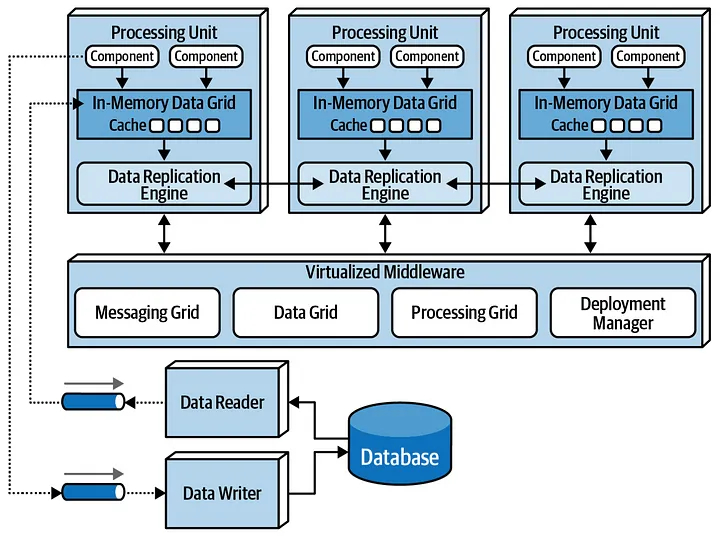
\includegraphics[height=0.8\textheight]{../../images/spaced-based_architecture.jpg}
			\label{fig:space-based_architecture}
		\end{figure}
	\end{frame}
	
	\begin{frame}{SBA Components (1)}
		\vspace{20pt}
		\begin{columns}[t]
			\begin{column}{0.55\textwidth}
				\textbf{Processing Unit (PU)}
				\begin{itemize}
					\item Contains application logic and local data cache.
					\item Can be replicated or partitioned.
					\item Operates independently.
				\end{itemize}
				
				\textbf{In-Memory Data Grid Cache}
				\begin{itemize}
					\item Provides fast in-memory access.
					\item Replaces main path database lookups.
				\end{itemize}
				
				\textbf{Data Replication Engine}
				\begin{itemize}
					\item Maintains data consistency across PUs.
					\item Handles automatic replication.
				\end{itemize}
			\end{column}
			
			\begin{column}{0.45\textwidth}
				\textbf{Virtualized Middleware}
				\begin{itemize}
					\item Infrastructure layer for shared services.
					\item Manages:
					\begin{itemize}
						\item Orchestration
						\item Messaging
						\item Synchronization
						\item PU deployment
					\end{itemize}
				\end{itemize}
			\end{column}
		\end{columns}
	\end{frame}
	
	\begin{frame}{SBA Components (2)}
		\vspace{20pt}
		\begin{columns}[t]
			\begin{column}{0.65\textwidth}
				\textbf{Processing Grid}
				\begin{itemize}
					\item Coordinates execution of tasks across multiple PUs.
					\item Enables efficient parallel task handling.
				\end{itemize}
				
				\textbf{Messaging Grid}
				\begin{itemize}
					\item Receives incoming requests.
					\item Routes them to the appropriate PU.
					\item Acts like a distributed load balancer.
				\end{itemize}
				
				\textbf{Data Grid}
				\begin{itemize}
					\item Distributed memory-based data store.
					\item Acts as shared space for PU communication.
					\item Supports partitioning and replication.
				\end{itemize}
			\end{column}
			
			\begin{column}{0.35\textwidth}
				\textbf{Deployment Manager}
				\begin{itemize}
					\item Starts/stops PU instances based on workload.
					\item Enables elastic scaling.
				\end{itemize}
				
				\textbf{Data Pump}
				\begin{itemize}
					\item Bridges PU and database.
					\item Sends data updates asynchronously.
				\end{itemize}
			\end{column}
		\end{columns}
	\end{frame}
	
	\begin{frame}{SBA Components (3)}
		\vspace{20pt}
		\begin{columns}[t]
			\begin{column}{0.5\textwidth}
				\textbf{Data Reader}
				\begin{itemize}
					\item Retrieves data from the database.
					\item Used mainly for cache recovery or reinitialisation.
				\end{itemize}
				
				\textbf{Data Writer}
				\begin{itemize}
					\item Receives updates from the Data Pump.
					\item Writes them to the database for persistence.
				\end{itemize}
			\end{column}
			
			\begin{column}{0.5\textwidth}
				\textbf{Database}
				\begin{itemize}
					\item Serves as the system of record.
					\item Not accessed in real-time processing flow.
					\item Updated indirectly and asynchronously.
				\end{itemize}
			\end{column}
		\end{columns}
	\end{frame}
	
	\begin{frame}{Request Flow in SBA (1)}
		\vspace{20pt}
		\begin{columns}[t]
			\begin{column}{0.5\textwidth}
				\textbf{Client Entry and Middleware}
				\begin{itemize}
					\item Requests enter through a web gateway or load balancer.
					\item Forwarded to the \texttt{virtualized middleware}.
					\item \texttt{Messaging grid} identifies the suitable \texttt{Processing Unit (PU)}.
				\end{itemize}
				
				\textbf{PU Selection}
				\begin{itemize}
					\item \texttt{Messaging grid} routes each request to an active PU.
					\item The selected PU processes the request independently.
				\end{itemize}
			\end{column}
			
			\begin{column}{0.5\textwidth}
				\textbf{Autonomous PU Structure}
				\begin{itemize}
					\item Each \texttt{PU} combines:
					\begin{itemize}
						\item Application logic (web/backend)
						\item In-memory cache (\texttt{in-memory data grid})
						\item Data replication engine
					\end{itemize}
					\item Operates independently from the database.
				\end{itemize}
				
				\textbf{Shared Memory}
				\begin{itemize}
					\item Uses distributed \texttt{data grid} as shared memory space.
					\item Enables fast access and consistent state sharing.
				\end{itemize}
			\end{column}
		\end{columns}
	\end{frame}
	
	\begin{frame}{Request Flow in SBA (2)}
		\vspace{20pt}
		\begin{columns}[t]
			\begin{column}{0.6\textwidth}
				\textbf{Data Update Handling}
				\begin{itemize}
					\item If a PU updates data, it becomes the owner of the latest version.
					\item The update is passed to the \texttt{data pump}.
					\item \texttt{Data pump} forwards it to the \texttt{data writer}.
					\item \texttt{Data writer} asynchronously persists the update in the database.
				\end{itemize}
				
				\textbf{No Direct DB Access}
				\begin{itemize}
					\item PUs do not access the database directly during processing.
					\item This improves throughput and eliminates bottlenecks.
				\end{itemize}
			\end{column}
			
			\begin{column}{0.4\textwidth}
				\textbf{Fallback with Data Reader}
				\begin{itemize}
					\item \texttt{Data reader} is used in recovery scenarios:
					\begin{itemize}
						\item PU failure
						\item Full cache reinitialisation
					\end{itemize}
					\item Reads from the database and populates PU memory.
				\end{itemize}
				
				\textbf{Eventual Consistency}
				\begin{itemize}
					\item Supports asynchronous updates with strong eventual consistency.
					\item Reduces latency and improves responsiveness.
				\end{itemize}
			\end{column}
		\end{columns}
	\end{frame}
	
	\begin{frame}{Request Flow in SBA (3)}
		\vspace{20pt}
		\begin{columns}[t]
			\begin{column}{0.5\textwidth}
				\textbf{Elastic Scaling}
				\begin{itemize}
					\item \texttt{Deployment manager} dynamically adjusts the number of PU instances.
					\item More PUs are launched during peak traffic.
					\item Idle PUs can be decommissioned automatically.
				\end{itemize}
				
				\textbf{Workload Adaptation}
				\begin{itemize}
					\item The system adapts to workload changes without downtime.
					\item Elasticity enables resource efficiency and cost optimisation.
				\end{itemize}
			\end{column}
			
			\begin{column}{0.5\textwidth}
				\textbf{Overall Benefits}
				\begin{itemize}
					\item Handles millions of requests in parallel.
					\item High fault tolerance and distributed load.
					\item Low-latency, high-throughput architecture.
					\item Promotes loosely coupled, scalable, and robust systems.
				\end{itemize}
				
				\vspace{10pt}
				SBA enables decentralised request handling with flexible scaling and efficient asynchronous persistence.
			\end{column}
		\end{columns}
	\end{frame}
	
	{
		\setbeamertemplate{navigation symbols}{}
		\setbeamertemplate{footline}{}
		\begin{frame}[plain]
			\begin{figure}
				\centering
				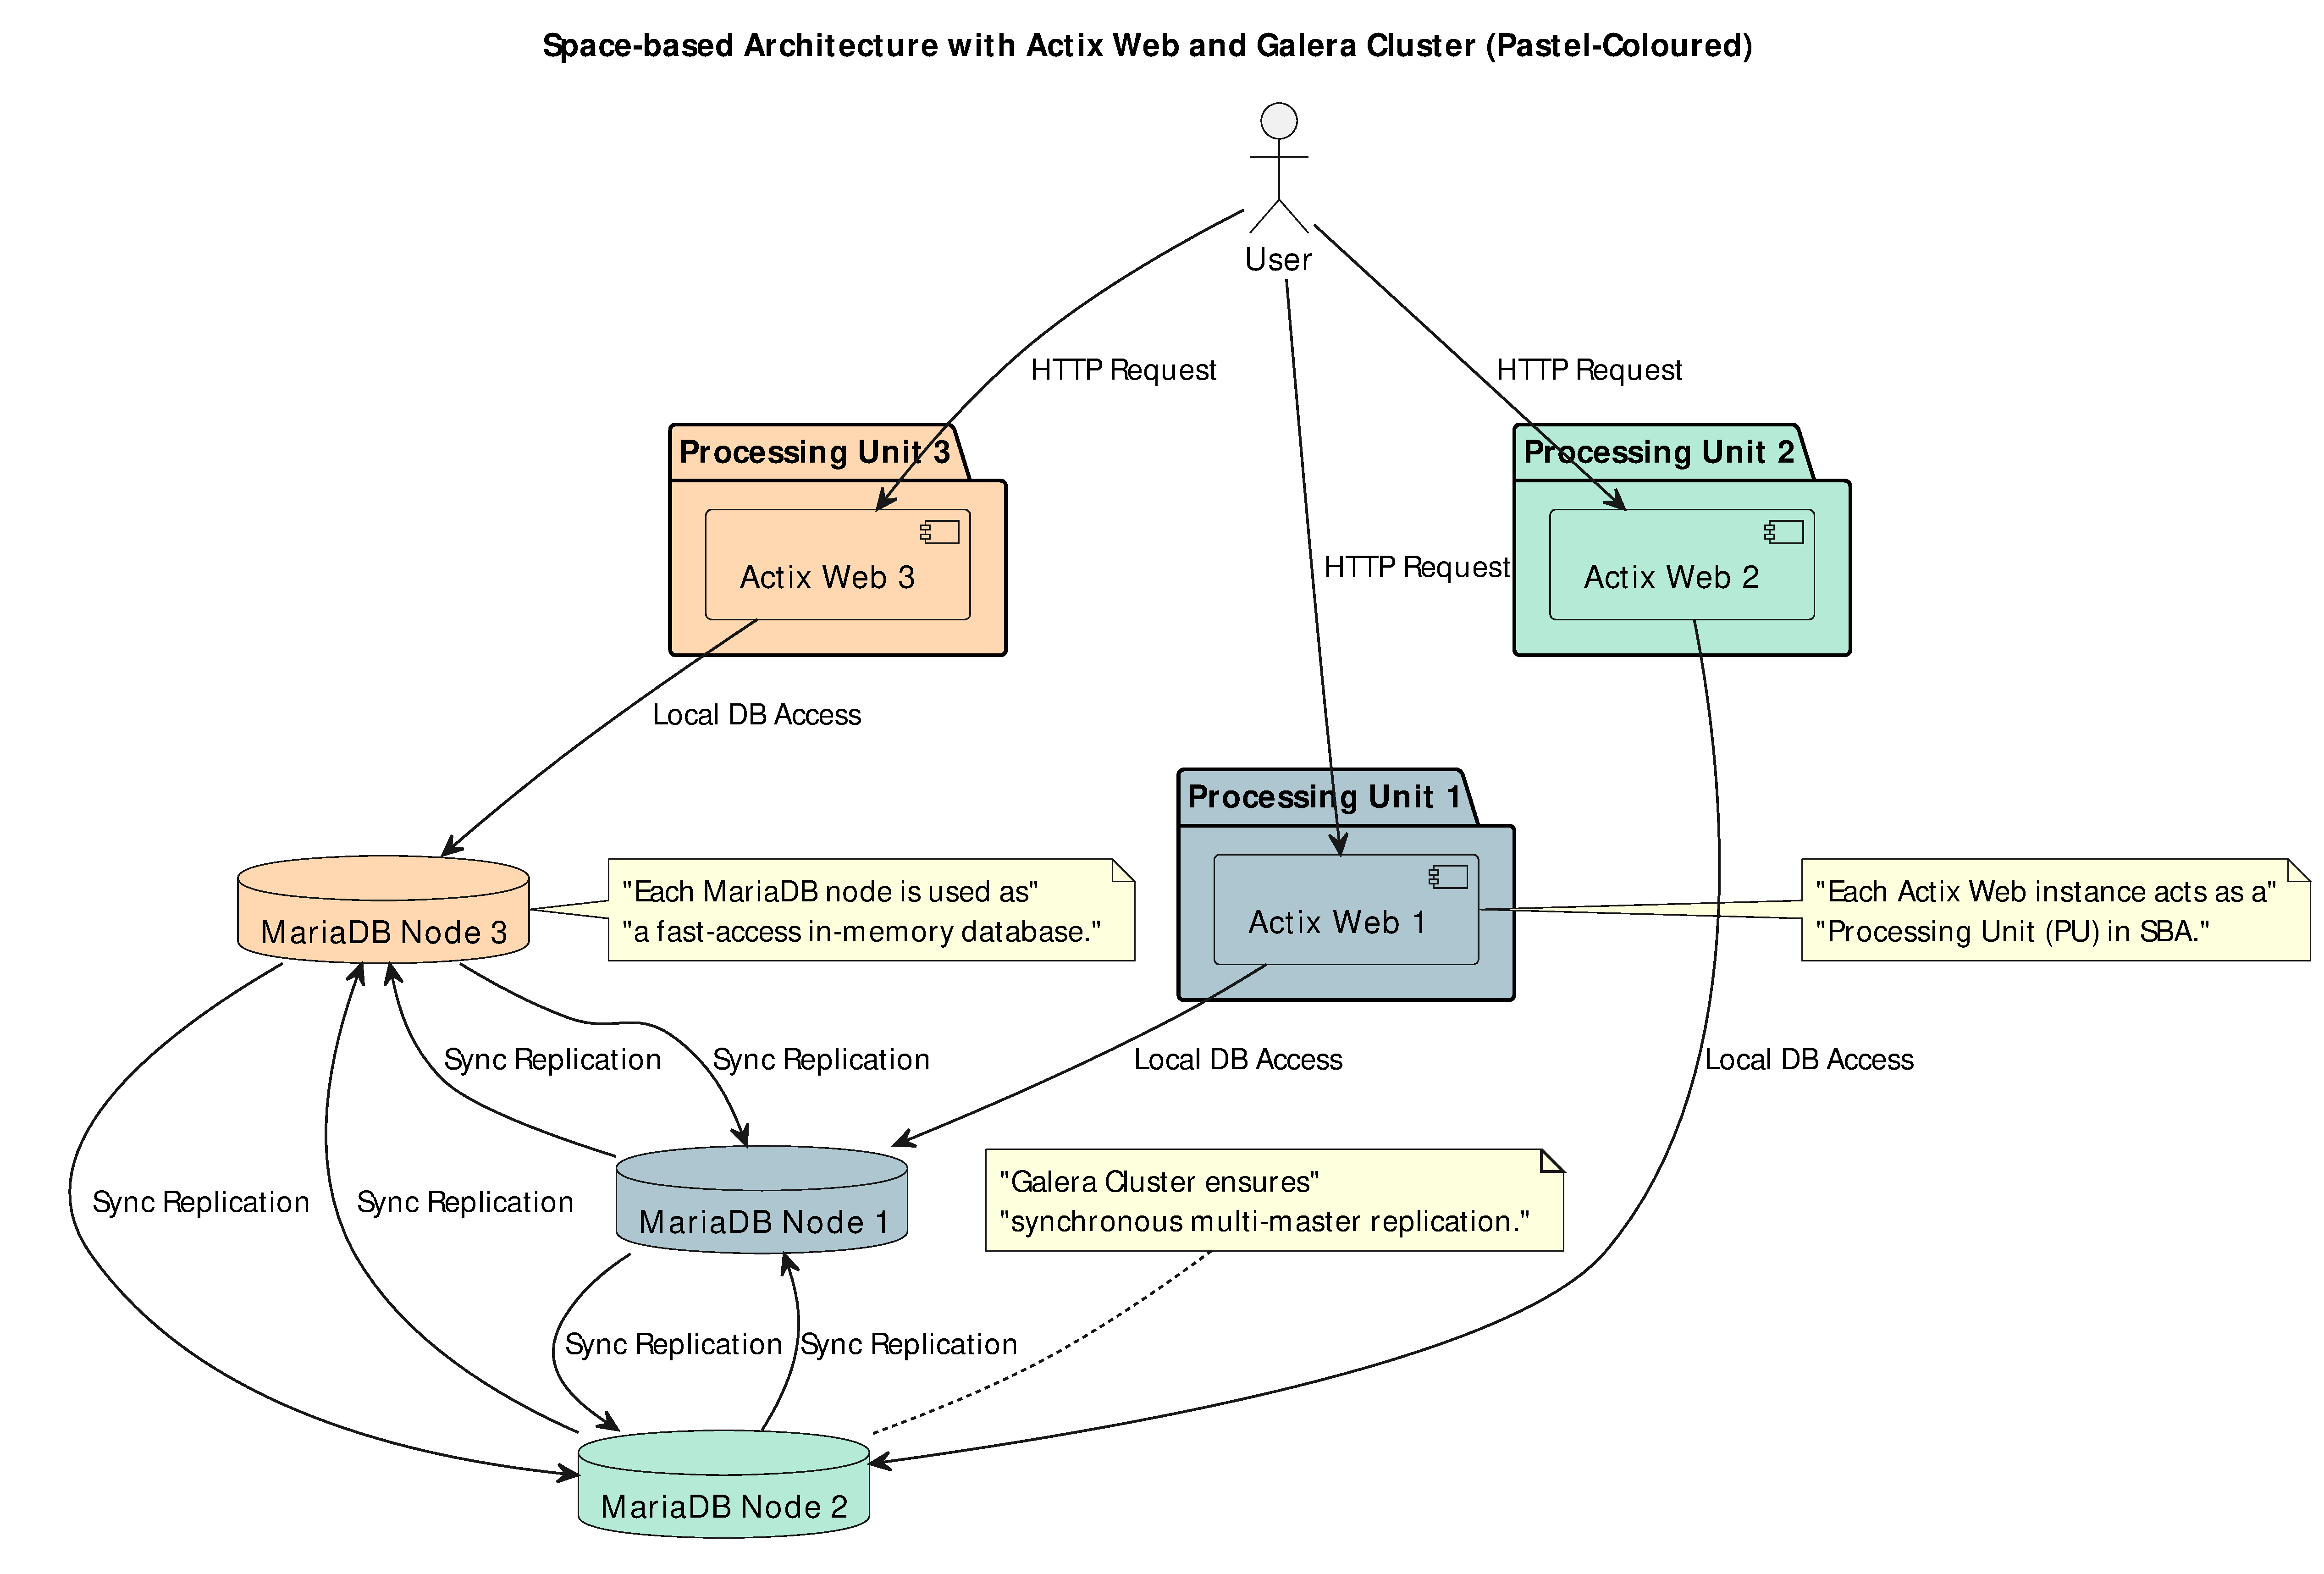
\includegraphics[height=\textheight]{../../images/out/space-based_architecture.pdf}
		\end{figure}	
		\end{frame}
	}
	
	
	
	\section{Conclusion}
	
	\begin{frame}{Conclusion: Space-based Architecture}
		\vspace{20pt}
		\begin{columns}[t]
			\begin{column}{0.5\textwidth}
				\textbf{Key Takeaways}
				\begin{itemize}
					\item SBA decouples data processing and storage from centralised components.
					\item Demonstrated using:
					\begin{itemize}
						\item \textbf{Galera Cluster} for synchronised data replication.
						\item \textbf{Actix Web} and \textbf{SQLx} for lightweight async web services.
					\end{itemize}
					\item Showcased distributed processing and shared memory usage.
					\item System remains consistent and operational despite node failures.
				\end{itemize}
			\end{column}
			
			\begin{column}{0.5\textwidth}
				\textbf{Modern Relevance}
				\begin{itemize}
					\item Highly relevant for real-time, cloud-native systems.
					\item Supports:
					\begin{itemize}
						\item Low latency
						\item Elastic scalability
						\item High availability
					\end{itemize}
					\item Prepares systems for dynamic and growing workloads.
					\item Empowers developers to design robust, efficient, and future-ready architectures.
				\end{itemize}
			\end{column}
		\end{columns}
	\end{frame}
	
	
\end{document}
